% Options for packages loaded elsewhere
\PassOptionsToPackage{unicode}{hyperref}
\PassOptionsToPackage{hyphens}{url}
%
\documentclass[
]{book}
\usepackage{amsmath,amssymb}
\usepackage{lmodern}
\usepackage{iftex}
\ifPDFTeX
  \usepackage[T1]{fontenc}
  \usepackage[utf8]{inputenc}
  \usepackage{textcomp} % provide euro and other symbols
\else % if luatex or xetex
  \usepackage{unicode-math}
  \defaultfontfeatures{Scale=MatchLowercase}
  \defaultfontfeatures[\rmfamily]{Ligatures=TeX,Scale=1}
\fi
% Use upquote if available, for straight quotes in verbatim environments
\IfFileExists{upquote.sty}{\usepackage{upquote}}{}
\IfFileExists{microtype.sty}{% use microtype if available
  \usepackage[]{microtype}
  \UseMicrotypeSet[protrusion]{basicmath} % disable protrusion for tt fonts
}{}
\makeatletter
\@ifundefined{KOMAClassName}{% if non-KOMA class
  \IfFileExists{parskip.sty}{%
    \usepackage{parskip}
  }{% else
    \setlength{\parindent}{0pt}
    \setlength{\parskip}{6pt plus 2pt minus 1pt}}
}{% if KOMA class
  \KOMAoptions{parskip=half}}
\makeatother
\usepackage{xcolor}
\IfFileExists{xurl.sty}{\usepackage{xurl}}{} % add URL line breaks if available
\IfFileExists{bookmark.sty}{\usepackage{bookmark}}{\usepackage{hyperref}}
\hypersetup{
  pdftitle={Workflows for processing microbial amplicon sequences},
  pdfauthor={Christian Krohn, PhD},
  hidelinks,
  pdfcreator={LaTeX via pandoc}}
\urlstyle{same} % disable monospaced font for URLs
\usepackage{longtable,booktabs,array}
\usepackage{calc} % for calculating minipage widths
% Correct order of tables after \paragraph or \subparagraph
\usepackage{etoolbox}
\makeatletter
\patchcmd\longtable{\par}{\if@noskipsec\mbox{}\fi\par}{}{}
\makeatother
% Allow footnotes in longtable head/foot
\IfFileExists{footnotehyper.sty}{\usepackage{footnotehyper}}{\usepackage{footnote}}
\makesavenoteenv{longtable}
\usepackage{graphicx}
\makeatletter
\def\maxwidth{\ifdim\Gin@nat@width>\linewidth\linewidth\else\Gin@nat@width\fi}
\def\maxheight{\ifdim\Gin@nat@height>\textheight\textheight\else\Gin@nat@height\fi}
\makeatother
% Scale images if necessary, so that they will not overflow the page
% margins by default, and it is still possible to overwrite the defaults
% using explicit options in \includegraphics[width, height, ...]{}
\setkeys{Gin}{width=\maxwidth,height=\maxheight,keepaspectratio}
% Set default figure placement to htbp
\makeatletter
\def\fps@figure{htbp}
\makeatother
\setlength{\emergencystretch}{3em} % prevent overfull lines
\providecommand{\tightlist}{%
  \setlength{\itemsep}{0pt}\setlength{\parskip}{0pt}}
\setcounter{secnumdepth}{5}
\usepackage{booktabs}
\usepackage{amsthm}
\makeatletter
\def\thm@space@setup{%
  \thm@preskip=8pt plus 2pt minus 4pt
  \thm@postskip=\thm@preskip
}
\makeatother
\usepackage{booktabs}
\usepackage{longtable}
\usepackage{array}
\usepackage{multirow}
\usepackage{wrapfig}
\usepackage{float}
\usepackage{colortbl}
\usepackage{pdflscape}
\usepackage{tabu}
\usepackage{threeparttable}
\usepackage{threeparttablex}
\usepackage[normalem]{ulem}
\usepackage{makecell}
\usepackage{xcolor}
\ifLuaTeX
  \usepackage{selnolig}  % disable illegal ligatures
\fi
\usepackage[]{natbib}
\bibliographystyle{apalike}

\title{Workflows for processing microbial amplicon sequences}
\author{\href{https://www.rmit.edu.au/contact/staff-contacts/academic-staff/k/krohn---christian}{Christian Krohn, PhD}}
\date{2022-07-05}

\begin{document}
\maketitle

{
\setcounter{tocdepth}{1}
\tableofcontents
}
\hypertarget{about-this-gitbook}{%
\chapter{About this GitBook}\label{about-this-gitbook}}


\includegraphics{./img/data.jpeg}

This GitBook contains workflows for students who want to get started with sequencing microbial amplicons on a Miseq instrument and then process and analyse ASV-based data. It is a compilation of workflows that I have gotten accustomed to during my PhD at La Trobe University with help of many amazing students and colleagues over the years. But it is by no means comprehensive.

One of the biggest hurdles for students that embark on sequencing environmental DNA for the first time, is the effort that is required to understand the various coding languages, file types and formats, packages or platforms that are involved (think Unix, Linux, Slurm, Qiime, R, RMarkdown, python, conda, ggplot, docker, GitHub, data instances\ldots) before they even can start looking at exploring the data for biological meaning and producing publishable output.

For example, this GitBook is made in \href{https://rstudio.com}{Rstudio}, using the \href{https://rstudio.com/wp-content/uploads/2016/03/rmarkdown-cheatsheet-2.0.pdf}{\texttt{rmarkdown} markup language}, rendered using the \href{https://bookdown.org/yihui/bookdown/get-started.html}{\texttt{bookdown} package}, and hosted on \href{https://github.com/}{GitHub}. It took me at least five years before I was ready to create and host this content for students. And even then I needed this awesome \href{https://cjvanlissa.github.io/gitbook-demo/index.html}{Bookdown template} from Dr.~Caspar van Lissa to get started with Bookdown. So it is really helpful to have something to start with.

It was not easy to get over the initial hurdles for me too, so I thought I'd try to compile my workflows. This may help students to get a head start but also helps to scrutinise my approach in the hope that others can point me to better ways of doing things.

\textbf{Browse to your level}

Everyone is at a different level in the journey to exploring microbial diversity. Some have absolutely no idea where to start and others have created their first phylogentic trees with ggtree or similar. The most important prerequisites are patience and persistence\ldots{} :). Just explore the different chapters and see where it takes you. In fact you will be amazed how much you can achieve with mininal coding knowledge.

\textbf{Get in touch}

We work at the Andy Ball lab, RMIT University, Bundoora, Melbourne. Email me or comment on the discussion section of the \href{https://github.com/chrismitbiz/ABlab-workflows/discussions/}{GitHub repository} for this GitBook. You will need to get a GitHub account to join the discussion. Its free.

\hypertarget{gettingstarted}{%
\chapter{Getting started}\label{gettingstarted}}

Prerequisites will be listed in each sub chapter separately.
Following a few general recommendations:

\textbf{Access to computational resources}

To process data you will need a personal computer or online computational resources with sufficient number of CPUs, working memory and storage. If you want to run most of the processing on a personal computer then I'd recommend a minimum of \textbf{4 CPUs, 16 Gb RAM and 500 Gb storage}. However, please note that some alignment tasks require more RAM, hence some of the steps (e.g.~taxonomic classifications) may require a more powerful resource. The advantage of using a personal computer is that you can frequently update the latest packages without relying on a university administrator to do that for you. Furthermore, with a personal computer you wont need to share with others, making it easier to run the packages without a workload manager.

Some university may provide their own access to a high performance computer (HPC) for staff and students and likely have certain packages pre-installed. In such cases a batch workload manger such as Slurm may be used, to manage multiple users trying to run computationally heavy jobs. This works fine too but its a bit of a hassle and I would use such an HPC only if really necessary, i.e.~smaller jobs on my personal computer and bigger jobs on the HPC.

I am not aware that RMIT University offers that type of service yet.

In Australia there is also the \href{https://ardc.edu.au/services/nectar-research-cloud/}{ARDC Nectar Research Cloud}, which provides free resources to Universities. This is basically like providing access to an online Linux computer with complete freedom to install any packages as if it was your own. If you are a student you can \href{https://dashboard.rc.nectar.org.au/}{create a trial account} with your student email address (Using your ID only; without the student.edu.au) and check out how it all works, albeit with limited resources. The Nectar service also provides \href{https://tutorials.rc.nectar.org.au/}{tuturials for starters}. However, to get serious with Nectar, you have to request more resources, which is a fairly straight-forward process. Check out the \href{https://support.ehelp.edu.au/support/solutions/articles/6000068044-managing-an-allocation}{eligibilities} and chat to your supervisor if you are interested.

There are also commercial options, which probably offer very similar type of services to Nectar.

In addition, there is the awesome \href{https://usegalaxy.org.au/}{Galaxy Australia platform}, which is an open web-based resource that also contains many tutorials and workflows specific to bioinformatics. Definitely worth checking that out too.

This workbook will be based on using the Nectar Research cloud.

\textbf{File storage}

Working with sequencing data may require you do handle large amounts of data. From experience, a run of a 600µl pool (6-10pM) of amplicons in 2x301 Miseq cycles may produce around 10-20 Gb of FASTQ files. \href{https://sapac.support.illumina.com/bulletins/2018/01/approximate-sizes-of-sequencing-run-output-folders.html}{Much more} can be expected for NextSeq runs or for long-read sequencing.

Once a Miseq run has finished it is typically available to download from the \href{https://basespace.illumina.com/dashboard}{Illumina Basespace} account. After a few runs, the data can accumulate quickly. Hence, \textbf{persistent storage space} is required. As long as you have the Basespace account you can keep a copy of the FASTQ file online. However, Basespace may delete your data if the account has been inactive for more than 6 months. Alternatively, data can be upload onto a public repository for persistent storage, such as the \href{https://www.ncbi.nlm.nih.gov/sra}{Sequence Reads Archives}. If you have access to a research cloud or commercial computational resources then you may store data on those. Personally, I prefer a 1TB solid state harddrive.

\textbf{Command Line}

Many of the tools used are managed through command line. Cloud servers are also accessed through command line. That means there is no graphical user interphase and all commands, including installation and running of packages are done through lines of codes on a simple window interphase. This window is called Terminal (Mac, Linux) or Command Prompt application (Windows). There are lots of online sources to help you get started with command line. One example here: \url{https://towardsdatascience.com/a-quick-guide-to-using-command-line-terminal-96815b97b955}

\textbf{Data storage browser}

To upload, download, move, rename files on any cloud computer or high performance computer (HPC) at your institution, you will also require a cloud storage browser, such as \href{https://docs.cyberduck.io/}{Cyberduck} (Mac) or \href{https://www.putty.org/}{PuTTY} (Windows).

\textbf{R and R studio}

R has become an essential research language. If you want to progress in research it is almost inevitable for you to learn. Just do it. :). Perhaps start here if you dont know where else to start: \url{https://education.rstudio.com/learn/beginner/}. It lists some great step-by-step tutorials on how to install R and Rstudio and then explains the basics.

If you are like me, then you simply copy and paste code from other sites and see what happens. This book should provide you with the required information to enable you to follow the workflows. In case you get stuck, you can either chat to me directly or write on the GitHub Discussion Page for this GitBook (\href{(https://github.com/chrismitbiz/ABlab-workflows/discussions/)}{chrismitbiz/ABlab-workflows/discussions/}).

At the same time you will want to do short courses (eg. from edX \href{https://www.edx.org/course/data-science-r-basics}{Data Science: R Basics}) that delve a little deeper into different data structures such as data frames, matrices, lists and the syntax to arrange stuff. Over time you understand what different lines of code mean and can trouble shoot when things don't work. And things often don't work. You will get used to troubleshooting code :).

\textbf{Environment managers}

Package and environment managers are extremely useful for your workflows. They help to install and run software packages such as qiime2, into individual `environments' independent of your operating system. The environment manager is installed once and from there you use it to install individual packages. The most commonly used environment manager is Conda. Learn more about it here: \url{https://docs.conda.io/projects/conda/en/latest/user-guide/getting-started.html}

Conda can be installed by either installing Anaconda or Miniconda. Boths works the same way. Anaconda requires 5 Gb of discspace and installs everything you can possibly need, while Miniconda is just the raw bones and lets you install things one by one.

Most of the commands to manage environments are done in command line using a terminal. There is also a graphical installer that makes handling the environments a little more visual. That would be my go to. Learn more here: www.anaconda.com

There are several other environment managers. We are also using \href{https://www.docker.com/}{Docker} in our work but the learning curve is a bit steeper so we wont get into it here.

\textbf{GitHub account}

This GitBook, including all its files, is hosted on one of my GitHub repositories (\url{https://github.com/chrismitbiz/ABlab-workflows}). If you have any comments you can ask a question on the Discussion Page of this repository. You require a GitHub account to do that. It is free.

\textbf{Workflows from other lab groups}

Searching for ``amplicon-sequencing'' under ``Topics'' on GitHub gave 37 results.

\begin{itemize}
\item
  nf-core/ampliseq\\
  On the top of that list is the \href{https://github.com/topics/amplicon-sequencing}{nf-core/ampliseq} pipeline developed by the nf-core community. It is based on a software called \href{https://www.nextflow.io/}{Nextflow} which allows to put different processes into a pipeline. This is great for doing things a little more reproducible but it requires you to be fairly knowledgeable with Linux, container software, config files etc.. Not great to learn stuff for beginners.
\item
  Tools-Microbiome-Analysis\\
  \href{https://microsud.github.io/Tools-Microbiome-Analysis/}{Tools-Microbiome-Analysis} is a websites containing a comprehensive list of R packages and, more importantly, tutorials related to analysis of microbial amplicons and ecology. Really good reference to go back to every now and then. \textbf{Highly recommended}.
\item
  grimmlab/MicrobiomeBestPracticeReview\\
  Essential paper to read (\href{https://academic.oup.com/bib/article/22/1/178/5678919}{Current challenges and best-practice protocols for microbiome analysis, 2021}) and a great \href{https://github.com/grimmlab/MicrobiomeBestPracticeReview}{workflow resource} on GitHub. \textbf{Essential read}. The Grimm lab in Munich published this paper as well as developed a python and R-based workflow that assists with the recommended best practices (amplicon as well as metagenomic workflows).
\item
  KasperSkytte/ampvis2\\
  \href{https://kasperskytte.github.io/ampvis2/articles/ampvis2.html}{Ampviz2} is an R-package to visualise and analyse 16S rRNA amplicon data. It is always more convenient to have packages that have the details and optics worked out for you. Like phyloseq, the ampviz2 package combines different tables from data (E.g. otu table, taxonomic table, phylogenetic tree, sample data etc) and then provides different functions to apply to that combined object to visualise the data.
\end{itemize}

\hypertarget{miseq-library-preps}{%
\chapter{Miseq library preps}\label{miseq-library-preps}}

\textbf{Some info on getting your run ready}

\textbf{Overview}

In our lab we usually prepare a 6-10 pM pool of libraries following the \href{https://sapac.support.illumina.com/content/dam/illumina-support/documents/documentation/chemistry_documentation/16s/16s-metagenomic-library-prep-guide-15044223-b.pdf}{16S Metagenomic Sequencing Library
Preparation} protocol from Illumina with 10\% Phix. \textbf{Download it, study it and refer to it throughout your labwork}. This protocol is not limited to 16S amplicons. You can use it for fungal (e.g.~ITS) amplicons too. In the last section there are also valuable tips for pre‐PCR and post‐PCR lab procedures. There is also some additional Illumina guidance here: \url{https://sapac.support.illumina.com/downloads/16s_metagenomic_sequencing_library_preparation.html}

The protocol encompasses the following steps (copied out of the protocol):
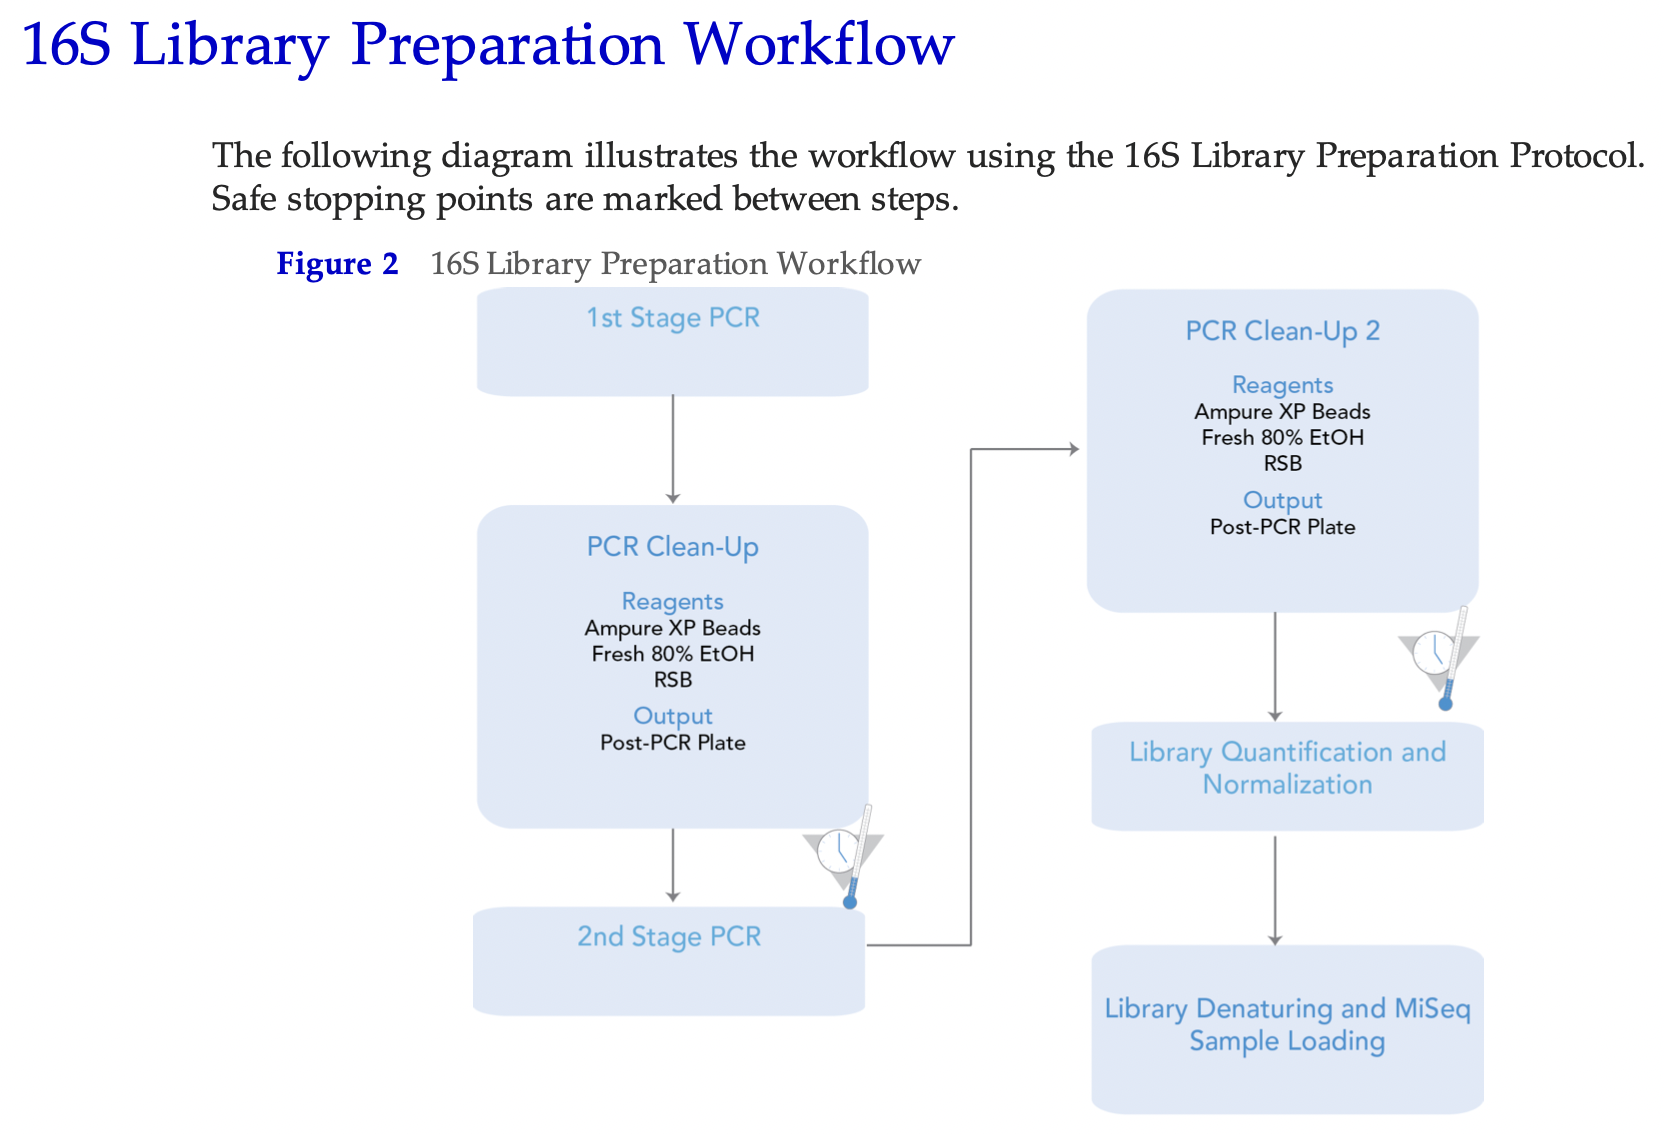
\includegraphics{./img/16Slibraryprotocolworkflow.png}

Please note that only \textbf{one amplicon target} should be sequenced in each run. That means it is not recommended to sequence for example two different 16S amplicons or one 16S amplicon plus an ITS amplicon. Sequencing different amplicon lengths will result in reduced quality as the the Miseq flowcell will preferentially cluster shorter fragments. However, it is not impossible. We have tried to run four different amplicons on one flowcell before, although with mixed results.

Labwork may take four weeks from DNA extraction to Miseq loading. Double that if you have not done it before. You probably realised that there is quite a bit of labwork required before you finally get FASTQ files and subsequent ASV/taxonomy tables to analyse - the ultimate goal here. The more samples are planned to be included into the pool, the more work and consumables are needed. Illumina recommends no more than 96 samples on one flowcell to get enough depths (i.e.~\textgreater{} 100,000 reads per sample). But we have sequenced around 196 samples on one flowcell before, which captured sufficient reads and diversity. This depends on how much detail and rare taxa you want to capture. The less samples you include, the more data and depth for each sample.

Also note that you will require over 20 boxes of tips (mostly 200 µl) for each 96-well plate, so plan your consumables ahead of time. Most of the tips will be used for the PCR clean ups.

After all steps in the above protocol are completed, the Miseq will be loaded with a 600 µl pool, followed by 56 hours of run-time for 2x301 cycles before FASTQ files are available for download from BaseSpace.

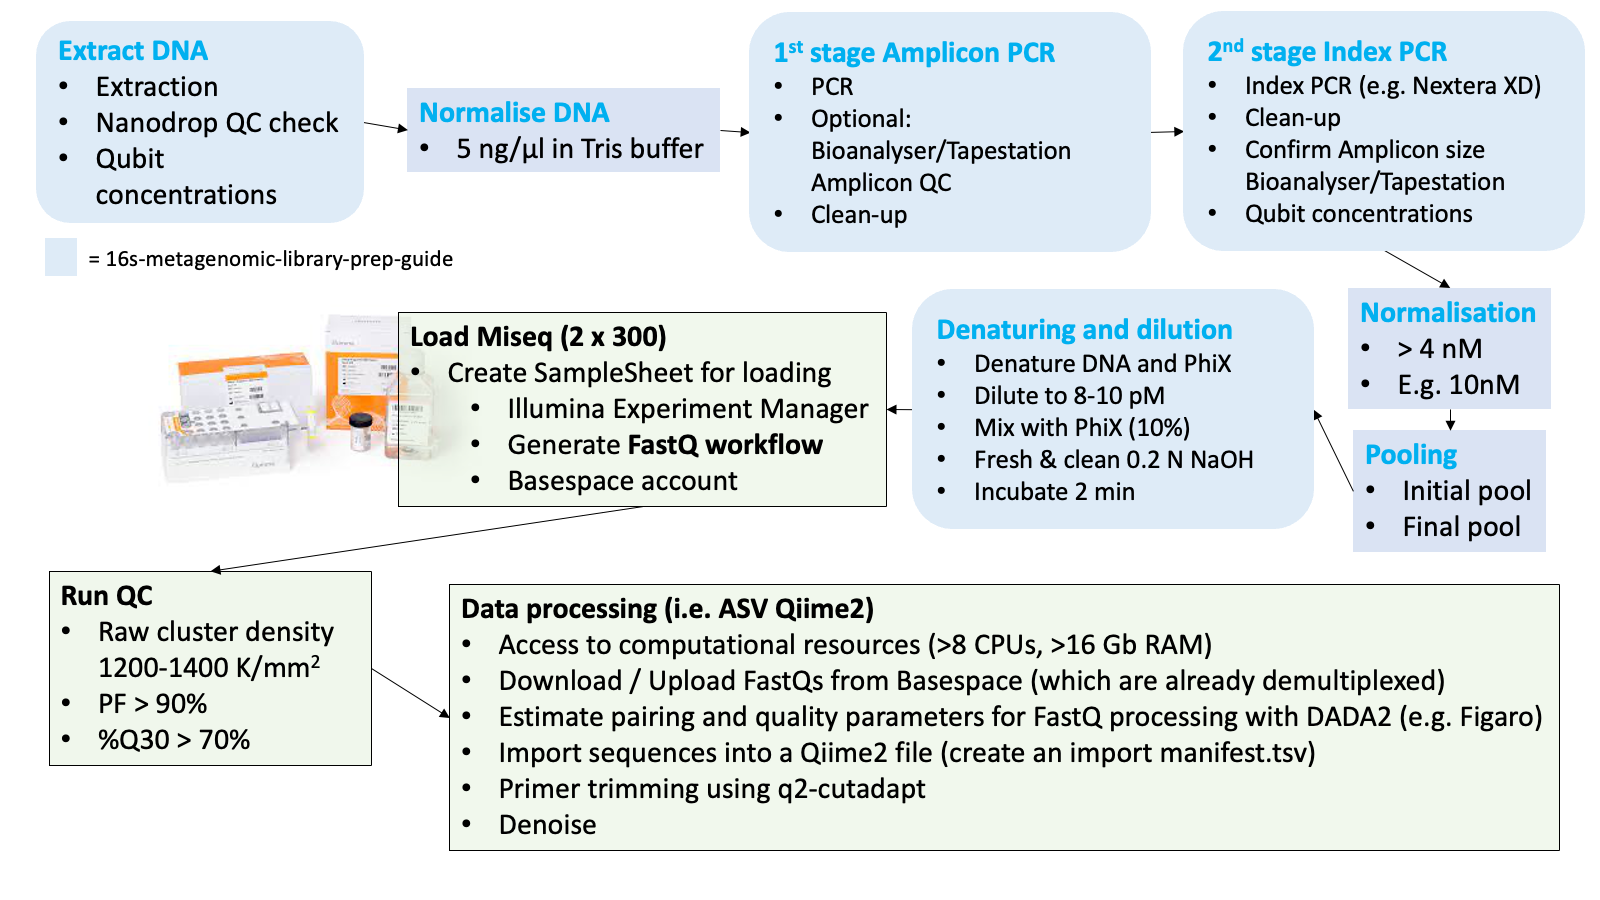
\includegraphics{./img/16s-library-prep-overview.png}

Throughout the 56 hours run you can check how things are tracking either on the BaseSpace website or the BaseSpace phone app. Understanding different QC metrics will help identifying potential problems with the pool or the instrument. It is important to note that this is a bit of a nerve-wrecking moment in the process, as it remains unclear until the metrics come through after around the 21st cycle, whether or not the run will be successful.\\
\strut \\
\strut \\

\textbf{1. DNA extraction}

\begin{figure}
\centering
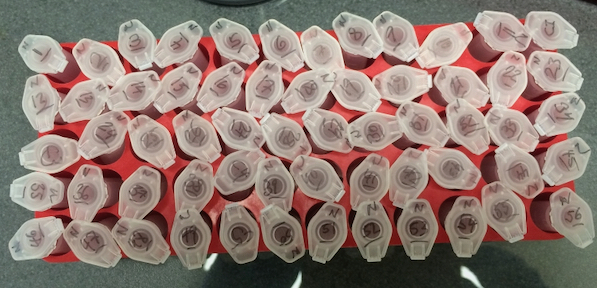
\includegraphics{./img/dna.jpeg}
\caption{``DNA extracts''}
\end{figure}

We commonly extract DNA from soils or from wastewater sludges using the \emph{DNeasy Powersoil Pro Kit} (Qiagen) for both, soil and sludge. It results in high quality DNA and includes a bead beating step to make sure the gram positive cells are sufficiently broken up. Although, I don't have evidence for that. In fact, please let us know on the \href{https://github.com/chrismitbiz/ABlab-workflows/discussions}{GitHub Discussion Page} for this GitBook if you have any comments on that as we are always looking for ways to improve things.

Soil

\begin{itemize}
\tightlist
\item
  For soils, the protocol of the extraction kit is followed, weighing in 0.25 g of soil and making sure to record the exact weights used.\\
\item
  Also make sure to measure the water content of the soil to be able to report DNA concentrations per dry weight of soil.
\end{itemize}

Sludge

\begin{itemize}
\tightlist
\item
  For DNA extraction of sludge, 0.5 ml is added into an empty 1.7 ml extraction tube (without extraction beads), then centrifuged at 5000 rpm for 5 minutes before removing the supernatent.
\item
  Extraction beads are then added and the Powersoil protocol followed.
\item
  Measure Total Solids (TS) of the sludge to report DNA concentrations per gram of TS.\\
  \strut \\
\end{itemize}

\textbf{2. DNA quality and concentration}

Once you have extracted DNA it is necessary to confirm its quality and concentration.

\begin{itemize}
\tightlist
\item
  Quality is assessed using a Nanodrop Spectrophotometer. You are aiming for \textbf{260/280 Ratio of 1.8 and a 260/230 Ratio of 2-2.2}. This is explained in the \href{https://dna.uga.edu/wp-content/uploads/sites/51/2019/02/Note-on-the-260_280-and-260_230-Ratios.pdf}{T042‐TECHNICAL BULLETIN}. The Nanopore also estimates DNA concentrations but it is not recommended to use these concentrations measurements to normalise DNA. It is more accurate and consistent with a Qubit Fluorometer.\\
\item
  DNA Concentrations are best measured using fluorescent dye-based methods such as the \textbf{Qubit Fluorometer}. It is easist to use the `\emph{1X}' assays such as the \emph{Qubit 1X dsDNA BR Assay Kit} or the \emph{Qubit 1X dsDNA HS Assay Kit}

  \begin{itemize}
  \tightlist
  \item
    Broad range (BR) Kit for quantifying extracted environmental DNA and afte the 2nd stage PCR.
  \item
    High Sensitivity (HS) Kit for quantifying the pool at the end.
  \end{itemize}
\end{itemize}

\begin{figure}
\centering
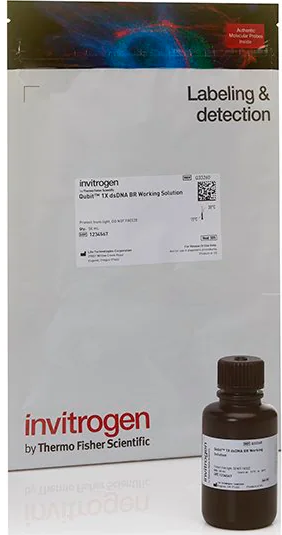
\includegraphics{./img/qubit.png}
\caption{``The ready-mix working solution for Qubit, which includes dye and buffer. No preparation/premixing required.''}
\end{figure}

\textbf{3. DNA normalisation}

The next step is to normalise all DNA extracts to 5 ng/µl.

\begin{itemize}
\tightlist
\item
  Dilute DNA to equal concentrations, either in a fresh batch of PCR-grade 10mM Tris buffer (pH 8.5) or in PCR-grade water\\
\item
  Set a pre-define DNA volume, say 2µl for all extracts, and add Tris or water as calculated with\\
  \[ C_1V_1 = V_2 C_2 \]\\
  \strut \\
\end{itemize}

\textbf{4. First and second PCR - Amplicon PCR and Indexing PCR}

Follow the \href{https://sapac.support.illumina.com/content/dam/illumina-support/documents/documentation/chemistry_documentation/16s/16s-metagenomic-library-prep-guide-15044223-b.pdf}{16S Metagenomic Sequencing Library
Preparation} Guide. Include a negative control and sequence that as well. This allows you to assess background and cross contamination. The whole workflow is best done in 96-well plates, using multi-channel pipettes to avoid indexing mistakes across wells.

Sample list and plate layout

Ensure that all sample IDs, plate-layout and each unique Illumina index carefully planned and printed out before you start your PCRs. Perhaps, stick the layout onto the Bio-safety cabinet where you do most of the pipetting and keep checking you are on the right well and sample. Label all plates even if you discard them afterwards. Labwork can be stressful and you need to trace all your steps across each well of the plate because otherwise you risk that you have indexed the wrong samples and it will become impossible to know which sample you have sequenced.

Primers

Any primers you order for the Miseq will have to include the \textbf{Illumina overhang adapter}. The sequence of the overhang adapter is added \textbf{in front} of the gene-specific primer sequences. There are two overhang adapters; one for the forward primers and one for the reverse primer. Check out the relevant information on primers from page 3 the 16S Metagenomic Sequencing Library Preparation Guide.

Clean-ups

It is worth doing the clean-ups in a separate deep-well plate (``MIDI'' plate, see consumables below) to avoid any blow-out of dried beads at the end of the clean-up. This process is explained in the above mentioned guide too. Tip: Handle the beads extremely carefully after the ethanol has dried. They blow out easily.

Index Kits

The index kits are expensive. Try to handle them with care and replace lids with the provided replacement lids, after every use. Multipipettes are absolutely essential to avoid loosing track on indexes used across the different wells on the plate. The use of the Illumina Plate Fixture comes in handy (see consumables below).

Amplicon QC

After the indexing PCR is cleaned it is recommended to run a gel on all samples to confirm that amplification was successful with enough DNA present and that it is the correct amplicon length. It also helps to identify any primer dimers, which may have to be cleaned out.

If you have access to a \textbf{Tapestation or a Bioanalyzer} in your lab, perhaps run a random subset of the indexed samples on one of these instruments, just to accurately confirm the average length of the amplicon. This average basepair length of the amplicon is important, as it is the basis for normalising your DNA to nM. In any case, after the index samples are normalised and pooled, it is highly recommended to run the pool on a Bioanalyser too. Otherwise it is too much guesswork in getting the concentrations right. This is further explained below.\\
Repeat any samples that failed, i.e.~that do not show any bands, and ensure you use the same indices.

\hfill\break

\textbf{5. Normalisation of Indexed amplicons}

After you finished all PCR work it is time to do another round of Qubitting and normalisation of all samples into a new 96-well plate. The final pool should be 4 nM but we prefer to normalise DNA to a higher concentration first, say 10 nM, then pool and then dilute the pool to 4 nM afterwards.\\
We are using a very handy excel sheet, which was kindly developed and provided by \href{https://scholars.latrobe.edu.au/sknowler}{Sarah Knowler} at La Trobe University to prepare and assist in normalisations, converting from ng/µl to nM using the formula:

\[ concentrations~(ng/µl)  \over 660 g/mol~x~average~library~size\]
Contact us if you would like to get a copy of this very handy library preparation excel sheet.

Some more information here: \url{https://support.illumina.com/content/dam/illumina-support/documents/documentation/system_documentation/miseq/miseq-denature-dilute-libraries-guide-15039740-10.pdf}. There's also a pooling calculator here \url{https://support.illumina.com/help/pooling-calculator/pooling-calculator.htm} which may be helpful with your calculations.\\
\strut \\

\textbf{6. Pooling}

\begin{itemize}
\item
  Pipette equal volumes of the normalised DNA into one 1.5 ml tube.\\
\item
  Measure its concentration using the High Sensitivity (HS) Qubit 1X dsDNA HS Assay Kit.\\
\item
  Assuming the pool was created wtih normalised concentration that are higher than 4 nM, then you will need to dilute the pool down to 4nM. In order to do so you will need to accurately measure the average basepair length of your pool. Do not rely on the ladder on a gel. Always get an accurate read. See next point.\\
\item
  Measure the average base pair lengths of the pool with a \textbf{Bioanalyzer or Tapestation}. Use at least three replicates. The average basepair length is then used to calculate the final concentration required in ng/µl to get a 4 nM pool.\\
\item
  Dilute the pool to the concentration in ng/µl that reflect 4 nM.

  \hfill\break
\end{itemize}

\textbf{7. Denaturing of pool and loading of the Miseq}

Now you are almost ready load the Miseq. The last steps are done right before you plan to load the instrument. First the pool DNA needs to be denatured, mixed with PhiX and then diluted further to your preferred loading concentration (6 - 10 pM). The final concentrations impact on cluster densities. That means you get more data with higher concentrations but that is at the expense of potential errors during sequencing at high cluster densities. I am still not quite sure what the ideal concentration is. Please let me know if you know more.

The key for the final steps are that..

\begin{itemize}
\tightlist
\item
  ..the reagent cartridge is properly thawed. Perhaps thaw in fridge 3 hours before starting the denaturing steps. Then put into icy water to ensure final and even thawing across the cartridge. Mix cartrige well at the end and ensure that no bubbles are visible before loading.\\
\item
  .. the 0.2 N sodium hydroxide (NaOH) is made fresh with biological grade NaOH. For example use the \emph{BioUltra, for molecular biology, 10 M NaOH in H2O} from Sigma Aldrich to make a 0.2 N solution (N = Normality but it is equal to Molarity here because there is only one OH in NaOH). I have used analytical-grade NaOH pellets as well, which worked but the RNAse free solutions are safer in terms of inhibitors etc..\\
\item
  ..that the pool is cooled down immediately in ice or icy water right after the 2 minutes in the 96 degrees C heatblock and pretty much immediately loaded into the Miseq. The Miseq has to be prepped beforehand (I.e. maintenance wash and sample sheet loaded).\\
\item
  a sample sheet (or so-called manifest file) is created beforehand using the Illumina Experiment Manager Software. This software assist in producing a \texttt{.csv} file that is then loaded into the Miseq instrument via a USB and ensures that the indexes you have used are linked to the relevant samples in your pool. Basically a list of sample IDs and index IDs. An example of a sample sheet from one of our runs is shown below.\\
  \textbf{IMPORTANT}: Make sure to specify the Workflow as \textbf{GenerateFastQ}.\\
\item
  you have a Illumina BaseSpace account.
\end{itemize}

\hfill\break

\begin{figure}
\centering
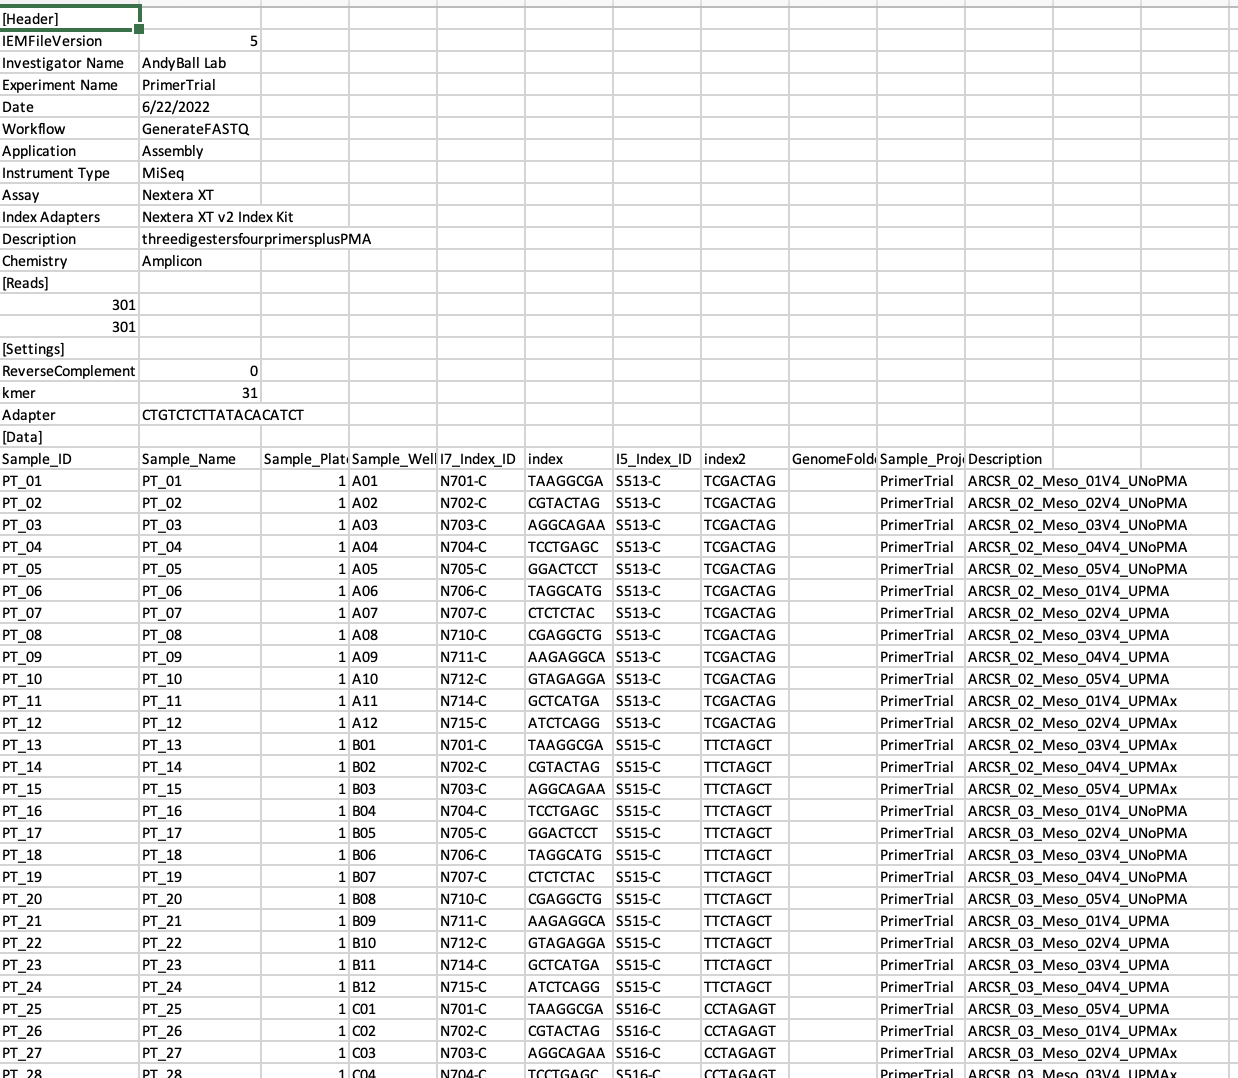
\includegraphics{./img/manifestfile.png}
\caption{``Example of a manifest file''}
\end{figure}

\textbf{8. Consumables}

All consumables and equipment required for the 16S Miseq library prep protocol are available from page 21 of the above mentioned \href{https://sapac.support.illumina.com/content/dam/illumina-support/documents/documentation/chemistry_documentation/16s/16s-metagenomic-library-prep-guide-15044223-b.pdf}{16S Metagenomic Sequencing Library
Preparation} Guide.\\
The \textbf{magnetic stand} for 96-well plates and the TruSeq Index \textbf{Plate Fixture Kit} are essential.

Here is what we typically include into our purchasing list. The combined total of the below list costs over AUD\$ 10,000.

\begin{table}

\caption{\label{tab:consumables}Example of a consumables list we typically include for a Miseq run}
\centering
\begin{tabular}[t]{llll}
\toprule
Equipment.consumables & Item.number & Supplier & Comment\\
\midrule
Qiagen Powersoil Pro test kit, 250 & \#47016 & Qiagen & \\
Primers & Various & E.g. Sigma & \\
Magnetic beads,  AMPure XP / JetSeq Clean & BIO-68031 & Meridian Life Sciences & For clean-up\\
KAPA HiFi Hotstart ready mix & KK2602, 6.25ml & Millennium Science & For PCR\\
MiSeq Reagent Kit v3 & MS-102-3003 & Illumina & Needs to be as fresh as possible\\
\addlinespace
Nextera XT Index Kit v2, Set A, B, C or D & FC-131-2003 & Illumina & One set (A, B, C or D) for 96 uniquely  indexed samples\\
PhiX control & FC-110-3001 & Illumina & \\
Qubit 1X dsDNA BR Assay Kit & Q33266 & Thermofisher & DNA and PCR-product quantiication\\
Qubit 1X dsDNA HS Assay Kit & Q33230 & Thermofisher & Pool quantification\\
Bioanalyzer Kit (HighSens or 1000 Kit) & 5067-4626 or 5067-1504 & Integrated Science Tech & \\
\addlinespace
Tween 20 & H5151 & Promega & For Miseq instrument wash\\
96-well, 0.2ml plates, non-skirted & AB0600 & Thermofisher & For PCR\\
96 Well 0.8mL Polypropylene Deepwel Plate & AB0859 & Thermofisher & For clean-up\\
Optical Plate Seals & V7840 & Promega & For PCR\\
0.5mL thin-walled PCR tubes & E4942 & Promega & For Qubit\\
\bottomrule
\end{tabular}
\end{table}

\hypertarget{from-basespace-to-qiime2-and-dada2}{%
\chapter{From BaseSpace to Qiime2 and DADA2}\label{from-basespace-to-qiime2-and-dada2}}

In this chapter you will learn how to process the FASTQ files that are generated from an amplicon sequencing run on a Miseq instrument. We are using Qiime2. Please also refer to the extensive documentation and tutorials available at \url{https://qiime2.org}. You can learn almost everything there.

\hfill\break

\textbf{Prerequisites}

\begin{itemize}
\item
  FASTQ files available to download on BaseSpace. Two for each sample. One for read 1 (R1) and another for read 2 (R2). For example, \texttt{PT-01\_S1\_L001\_R1\_001.fastq.gz} and \texttt{PT-01\_S1\_L001\_R2\_001.fastq.gz} contains all sequences for sample PT-01.
\item
  Personal computer or cloud computational resources with \textgreater{} 4 CPUS, \textgreater{} 16 RAM, \textgreater{} 100 GB storage recommended.\\
\item
  Cloud storage browser installed (example Cyberduck or PuTTYm see Chapter \ref{gettingstarted}).\\
\item
  Qiime2 installed. Always use the latest version.\\
\item
  All required files in correct format and file extension (see below).\\
\item
  The BaseSpace Downloader software (available on the BaseSpace page. You will be prompted to download once you go to your files).

  \hfill\break
\end{itemize}

\textbf{Download FASTQ files}

In this example, Fastq files were produced from sequencing 16SrRNA marker genes on an Illumina Miseq instrument. If you ran your own library on your own BaseSpace account, the files should be available to download from that BaseSpace account. If the run was created by another user, that person can invite you to the run, which gives you access to download the files too.

Log in to BaseSpace and into your project. Go to files, run and download FastQ. You will be asked to install a downloader software. Follow instructions accordingly.\\
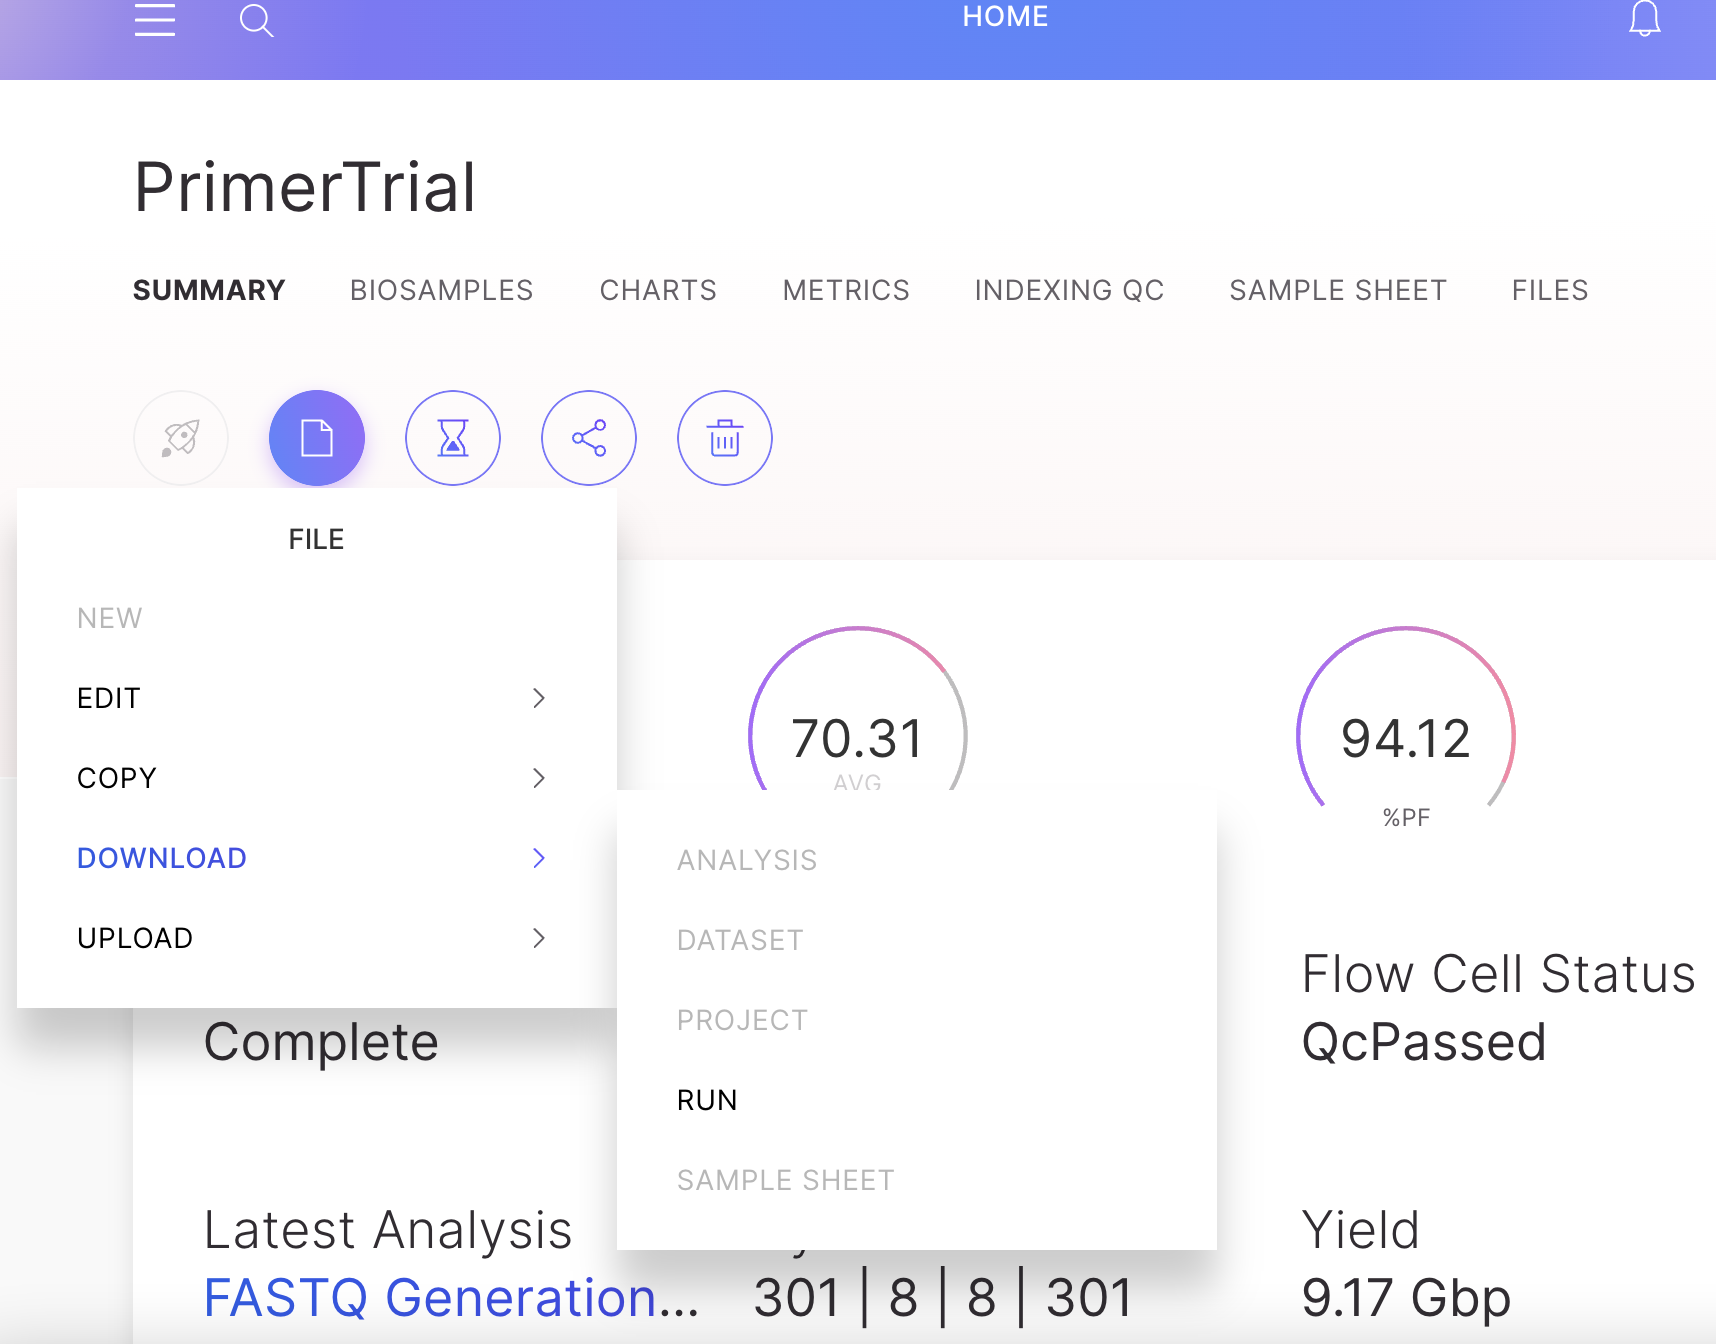
\includegraphics{./img/basespacedownload.png}

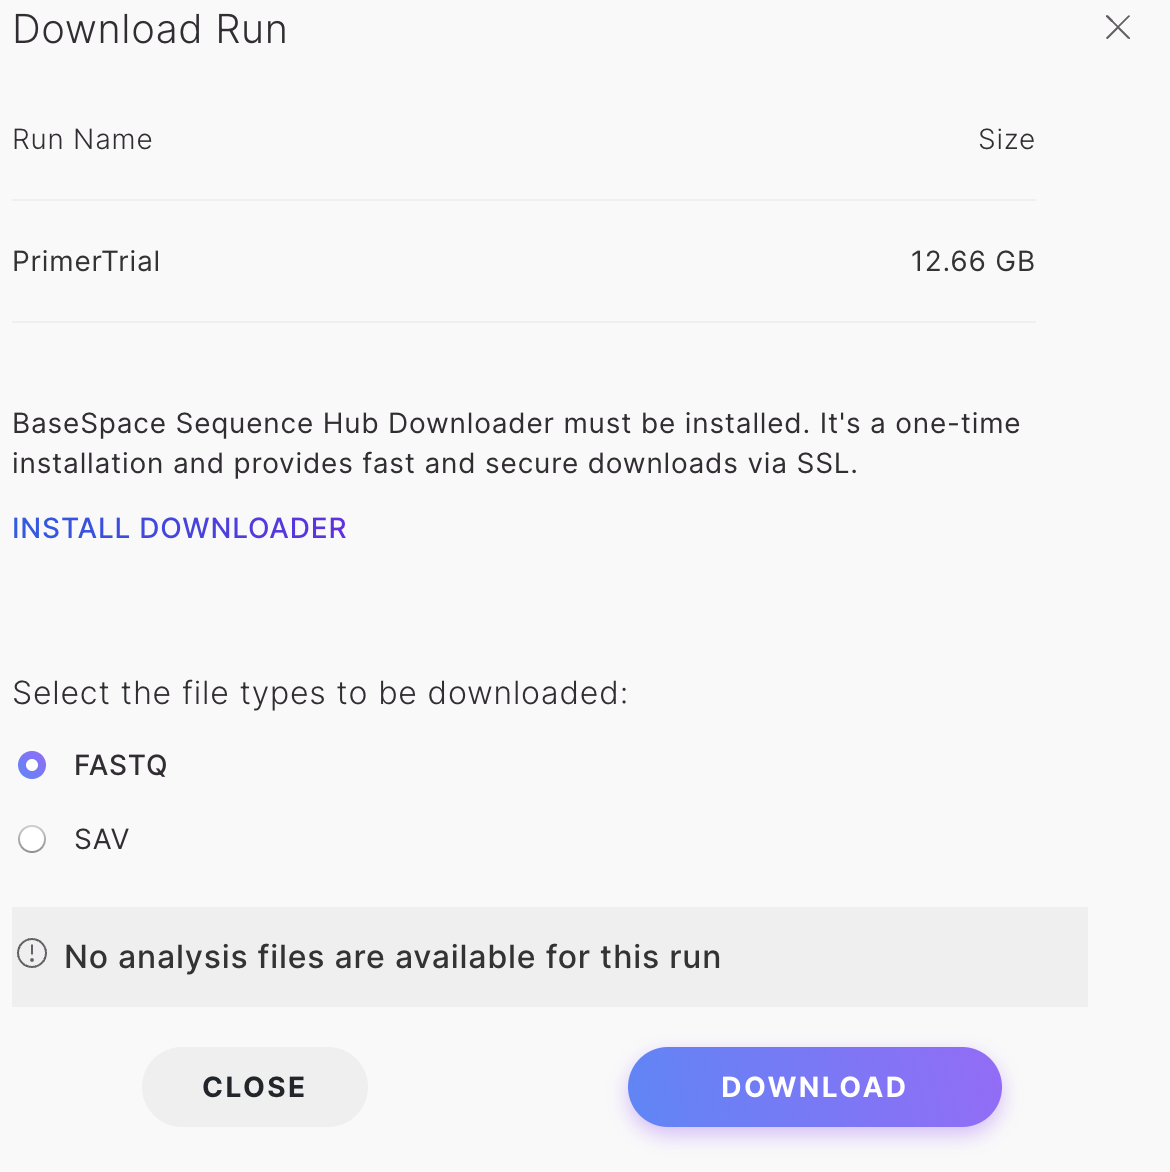
\includegraphics{./img/basespacedownload2.png}\\
\strut \\

The FASTQ files will come in separate folders for each sample. It is necessary to move all files into just ONE folder. That folder will then be used to import the sequences into a qiime object (described below).

\hfill\break

\textbf{Required Files}

\texttt{Qiimeimportmanifest.tsv} - A tab separated file with three columns where the first column is the sample ID (The exact same ID that was used in the manifest file for loading the Miseq). The second and third columns are the absolute paths to the forward and reverse FASTQ files, respectively. If you are working on a cloud computer then the FASTQ files should be uploaded to that, and the path needs to contain the full path to the relevant folder, including the full name of the file itself. If you process those files on your local drive then the paths need to change to your local folder containing the FASTQ files. In the below example table, the files are located on a Linux cloud computer (Nectar Research Cloud).

It might take some time to compile the import manifest. Each file path has to exact. However, in case you made a mistake in the file names etc, Qiime is generally pretty good at reporting where the error occured.

\begin{table}

\caption{\label{tab:qiimeimport}Example of a qiime import manifest.tsv file}
\centering
\fontsize{10}{12}\selectfont
\begin{tabular}[t]{l|l|l}
\hline
sample-id & forward-absolute-filepath & reverse-absolute-filepath\\
\hline
PT-01 & /pvol/Sequences/20220622\_PrimerTrial\_RMIT/PT-01\_S1\_L001\_R1\_001.fastq.gz & /pvol/Sequences/20220622\_PrimerTrial\_RMIT/PT-01\_S1\_L001\_R2\_001.fastq.gz\\
\hline
PT-02 & /pvol/Sequences/20220622\_PrimerTrial\_RMIT/PT-02\_S2\_L001\_R1\_001.fastq.gz & /pvol/Sequences/20220622\_PrimerTrial\_RMIT/PT-02\_S2\_L001\_R2\_001.fastq.gz\\
\hline
PT-03 & /pvol/Sequences/20220622\_PrimerTrial\_RMIT/PT-03\_S3\_L001\_R1\_001.fastq.gz & /pvol/Sequences/20220622\_PrimerTrial\_RMIT/PT-03\_S3\_L001\_R2\_001.fastq.gz\\
\hline
PT-04 & /pvol/Sequences/20220622\_PrimerTrial\_RMIT/PT-04\_S4\_L001\_R1\_001.fastq.gz & /pvol/Sequences/20220622\_PrimerTrial\_RMIT/PT-04\_S4\_L001\_R2\_001.fastq.gz\\
\hline
PT-05 & /pvol/Sequences/20220622\_PrimerTrial\_RMIT/PT-05\_S5\_L001\_R1\_001.fastq.gz & /pvol/Sequences/20220622\_PrimerTrial\_RMIT/PT-05\_S5\_L001\_R2\_001.fastq.gz\\
\hline
PT-06 & /pvol/Sequences/20220622\_PrimerTrial\_RMIT/PT-06\_S6\_L001\_R1\_001.fastq.gz & /pvol/Sequences/20220622\_PrimerTrial\_RMIT/PT-06\_S6\_L001\_R2\_001.fastq.gz\\
\hline
\end{tabular}
\end{table}

\hfill\break

\texttt{samplesheet.tsv} - file containing sample metadata. This file should contain all other environmental measurements you may have done on each sample (pH, EC\ldots), which you want to relate to microbial taxonomy and composition. The same file and format will be used to import metadata into the R package Phyloseq later too.

\begin{table}

\caption{\label{tab:metadata}Example of a samplesheet.tsv file}
\centering
\fontsize{10}{12}\selectfont
\begin{tabular}[t]{l|l|l|l|l|l|l}
\hline
\#SampleID & \#Sludge & WWTP & SludgeType & PMA\_treat & Rep\_bio & Sludgecollection\\
\hline
\#q2:types & categorical & categorical & categorical & categorical & numeric & categorical\\
\hline
PT-01 & 1 & ETP5 & Meso & NoPMA & 1 & 9/5/2022\\
\hline
PT-02 & 1 & ETP5 & Meso & NoPMA & 2 & 9/5/2022\\
\hline
PT-03 & 1 & ETP5 & Meso & NoPMA & 3 & 9/5/2022\\
\hline
PT-04 & 1 & ETP5 & Meso & NoPMA & 4 & 9/5/2022\\
\hline
PT-05 & 1 & ETP5 & Meso & NoPMA & 5 & 9/5/2022\\
\hline
\end{tabular}
\end{table}

\hfill\break

IMPORTANT: Create the \texttt{.tsv} file as a tab separated \texttt{.csv} file in Excel first and then manually change the file name from \texttt{.csv} to \texttt{.tsv}. Not sure how else to easily build the \texttt{.tsv} file.

\hfill\break

\texttt{scriptfile.txt} - A text file that contains your qiime2 scripts. Example below. Code is compiled here and then only the file itself is executed to run any commands in that text. The hash (\#) in front of any line of code stops it from being executed. That means all code is normally `hashed'. If one wants to run the code the lines are `un-hashed' and the text file is executed in the command line to run the `un-hashed' code. On the Linux cloud computer the command would be: \texttt{sh\ scriptfile.txt}.

Note that a script file is meant to make life easy and the process replicable. But you could run each of the processes directly by adding the commands into the terminal without a script file.

\begin{figure}
\centering
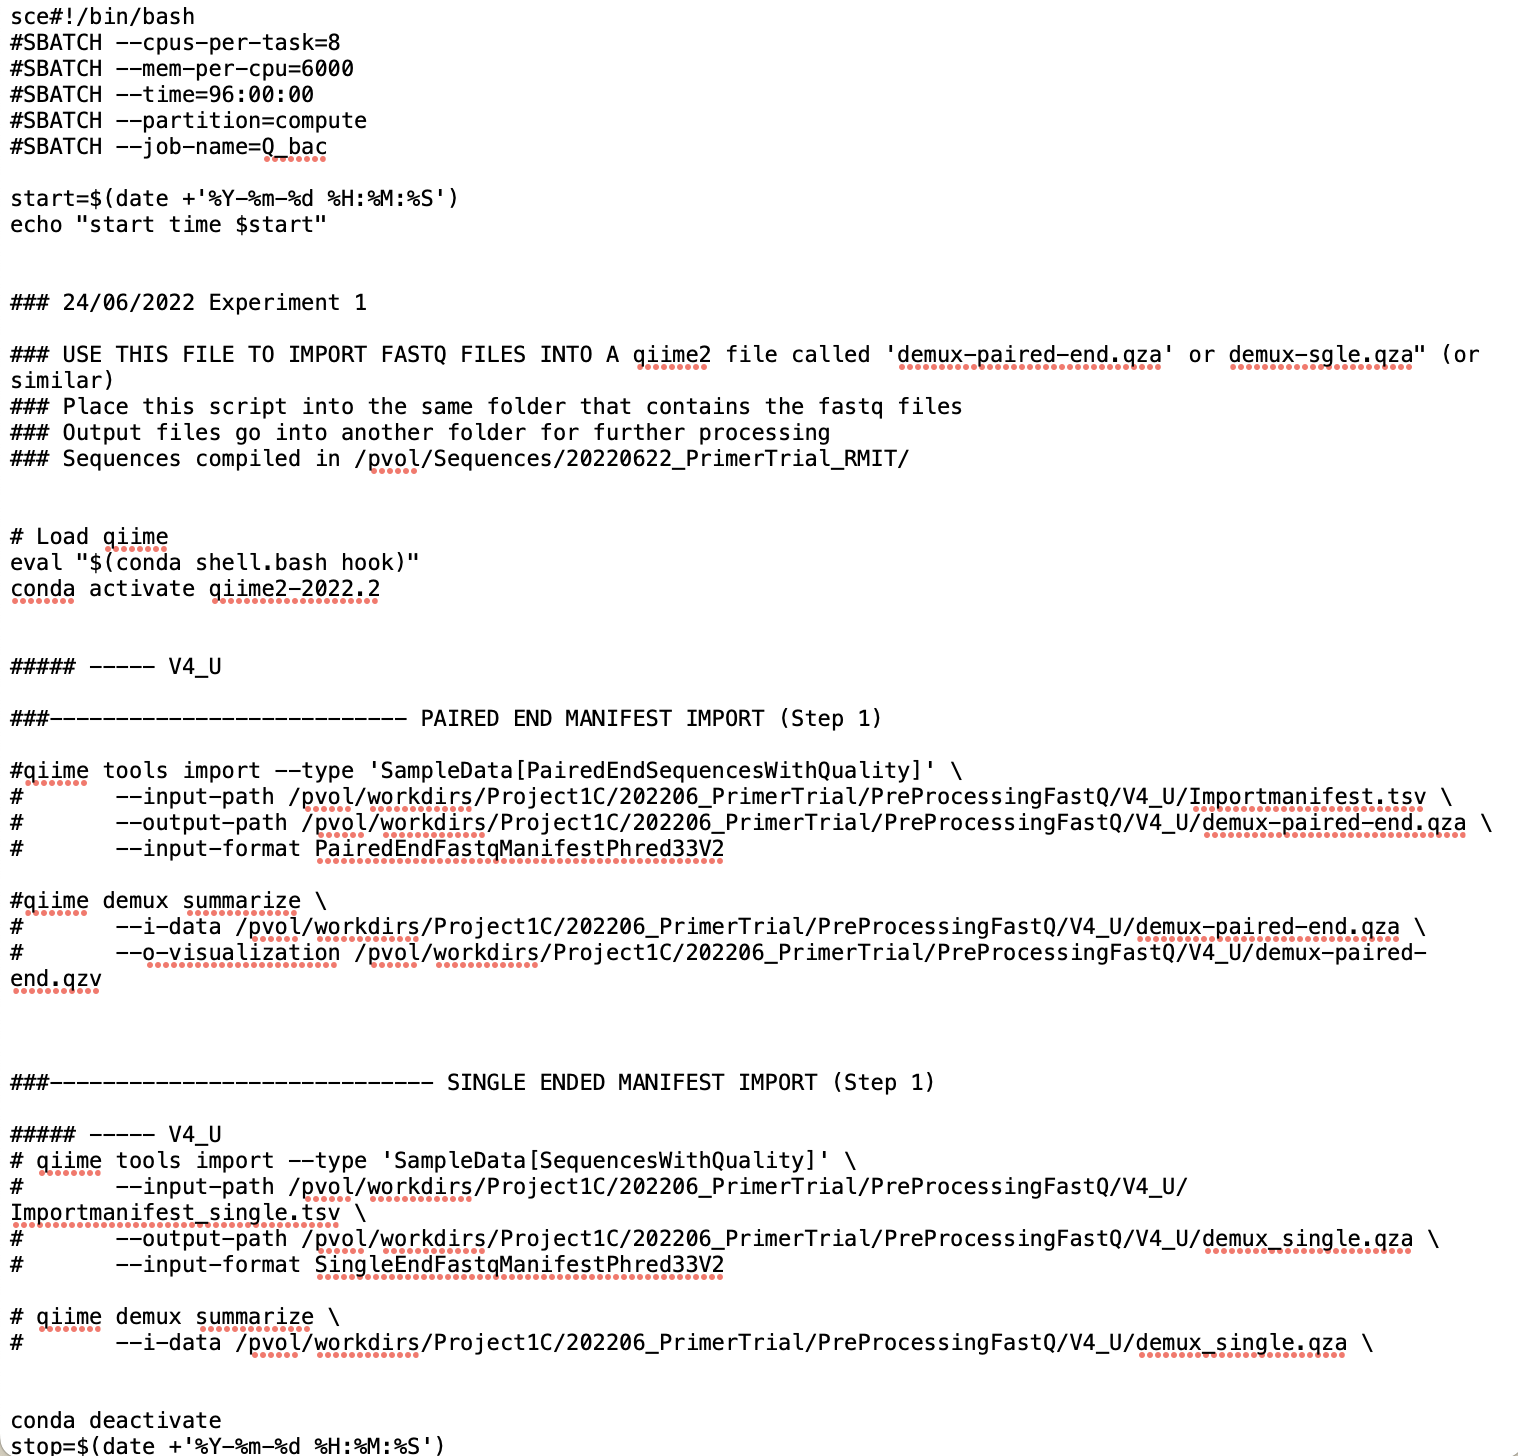
\includegraphics{./img/scriptfile.png}
\caption{``Example of a scriptfile.txt''}
\end{figure}

\hfill\break

Briefly on script files for cloud-based high performance computers (HPC) that are using Slurm to manage multiple user runs. If the HPC at your institution is using Slurm, then the script file has to be called with \texttt{sbatch\ scriptfile.txt}. The script files for HPCs using slurm contains a header that determins the allocations (number of CPUs, RAM etc..) for your task. The first lines of the .txt file typically look similar to this:

\begin{verbatim}
#!/bin/bash
#SBATCH --cpus-per-task=6
#SBATCH --mem-per-cpu=6000
#SBATCH --time=24:00:00
#SBATCH --partition=compute
#SBATCH --job-name=Q_fun
\end{verbatim}

Commands, such as this:

\begin{verbatim}
echo "Starting at: $(date)"
echo "Finished at: $(date)"
\end{verbatim}

.. are less important but help to report the start and end times of the executed commands from beginning (where the \texttt{echo} command is placed at the beginning of the script) to end (\texttt{echo}\ldots{} placed at the end of the script) into the Terminal Windows. They dont affect the qiime commands in any way.

Slurm and \texttt{sbatch} are not needed if you manage your own computer or your `own' cloud computer. In the example below we are using a Linux cloud computer, provided by the Nectar Research Cloud so we dont need Slurm.

\hfill\break

\textbf{Paired end manifest import (Step 1)}

Go to the folder that contains all the FASTQ files (all files in one folder). I.e. in Unix/Linux use \texttt{cd\ path/to/folder/} to navigate to it. The scriptfile.txt should also be located here. The following qiime command that will look for the files and then create a qiime object using the sequences found in each FASTQ file. The \texttt{-\/-output-path} instructs qiime where to place and how to name the output file, here demux-paired-end.qza is placed into the same directory.\\
Remove any \# in front of your code (already removed in the below example) and execute the scriptfile.txt with \texttt{sh\ scriptfile.txt} (or \texttt{sbatch\ scriptfile.txt} in case you are using Slurm).

\begin{verbatim}
qiime tools import --type 'SampleData[PairedEndSequencesWithQuality]' \
  --input-path Qiimeimportmanifest.tsv \
  --output-path demux-paired-end.qza \
  --input-format PairedEndFastqManifestPhred33V2
\end{verbatim}

\hfill\break

\textbf{Cutadapt (Step 2)}

If all goes well you should now have a demux-paired-end.qza file in the same directory as your FASTQ files , which contains all your sequences. You could move demux-paired-end.qza to another folder and continue all other steps there if you wish. The FASTQ files are not needed anymore. Dont forget to move your script file to where it is most convenient for executing the commands. If you moved the demux-paired-end.qza to another folder it is probably easiest to also move the script file that the same directory (or create a second script file containing the remaining commands).

Go to the folder containing demux-paired-end.qza and use cutadapt to trim out the primer sequences. Unhash relevant lines in your script file, which should be located in the same folder. Run \texttt{sh\ scriptfile.txt}.

In this example we used the V4 primers. Change primer sequence to the exact primers that you used in the amplicon PCR.

\begin{verbatim}
qiime cutadapt trim-paired \
  --i-demultiplexed-sequences demux-paired-end.qza \
  --p-front-f GTGYCAGCMGCCGCGGTAA \
  --p-front-r GGACTACNVGGGTWTCTAAT \
  --o-trimmed-sequences trimmed_demux-paired-end.qza
\end{verbatim}

\hfill\break

\textbf{Visualise the output with a .qzv file}

The .qza files can be visualised by `converting' them into .qzv files.\\
Here we take the trimmed\_demux-paired-end.qza and create a trimmed\_demux-paired-end.qzv.\\
\textbf{NOTE:} View any .qzv file on \url{https://view.qiime2.org}. Drag and drop the qzv file into the browser window and inspect the results.

\begin{verbatim}
qiime demux summarize \
  --i-data trimmed_demux-paired-end.qza \
  --o-visualization trimmed_demux-paired-end.qzv
\end{verbatim}

Go to \url{https://view.qiime2.org} and drag and drop to visualise your .qzv file in the browser.

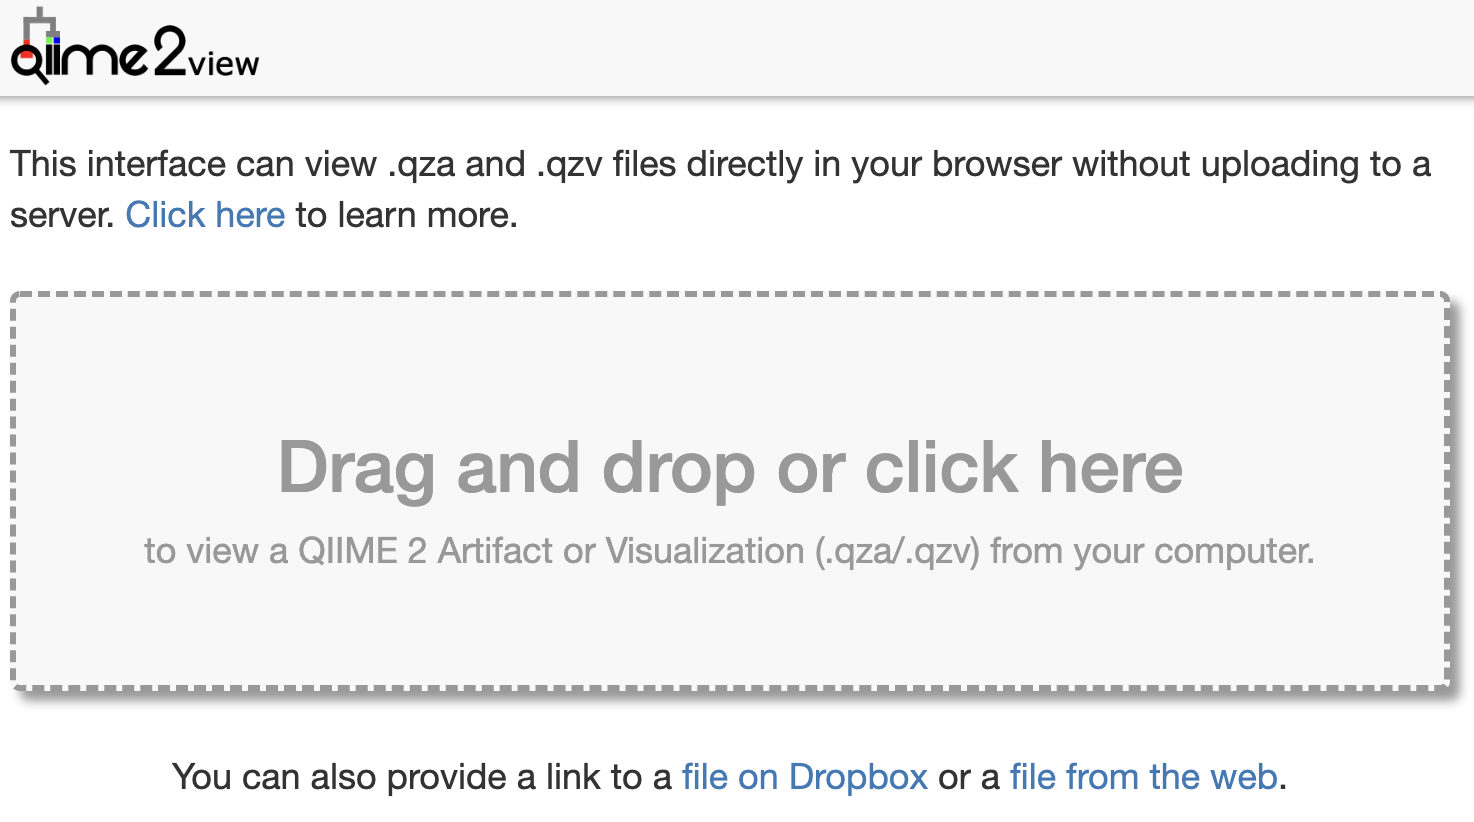
\includegraphics{./img/viewqiime.png}\\

\textbf{STOP HERE}. Inspect the visualisation and decide on location and maximum expected error.\\
From the output decide where to truncate the forward and reverse reads with \texttt{p-trunc-len-f}, \texttt{p-trunc-len-r},\texttt{-\/-p-max-ee-f} and \texttt{-\/-p-max-ee-r} in DADA2 below.

It can take some trial and error to get these setting right. We are using a docker-based package called FIGARO to help us estimate those parameters (Not shown here). But essentially you want to capture high quality reads and be confident about the Amplicon Sequence Variants (ASV), while also capture sufficent depth of ASVs and reads without unnecessarily filtering out too much. In the below example, we have trimmed the forward reads at 272 base pairs with a maximum expected error (max-ee) of 2 (which is the default) and the reverse reads at 151 with a max-ee of 3. I think it is o.k. to relax the max-ee for the reverse reads (which are ALWAYS lower in quality) as I feel more confident about the fact that the reverse reads are paired with the forward reads. Pairing in itself provides increased confidence that the reads do in fact represent a biological relevant sequence. As always please comment on our \href{https://github.com/chrismitbiz/ABlab-workflows/discussions/}{GitHub discussion page} if you have any suggestions here. Thanks!

A minimum overlap between the forward and reverse primer of 20 base pairs is recommended. To overlap can be calculated as following:

length forward read + length reverse read - length amplicon - trimmed basepairs forward read - trimmed basepairs reverse reads = overlap

So, for example, if we picked \texttt{-\/-p-trunc-len-f\ 272} and \texttt{-\/-p-trunc-len-r\ 151}, we get
\[301 + 301 - 292 - 29  - 150 = 131~bp~overlap\]

\hfill\break

In cases where the quality of the reverse reads is very poor, or the amplicon is too long for pairing to work, it is also acceptable to import, trim and denoise only the forward reads. The V4 primer of this example, is nice and short at 292 basepairs, so is great for pairing even at lower reverse-read qualities.

\begin{figure}
\centering
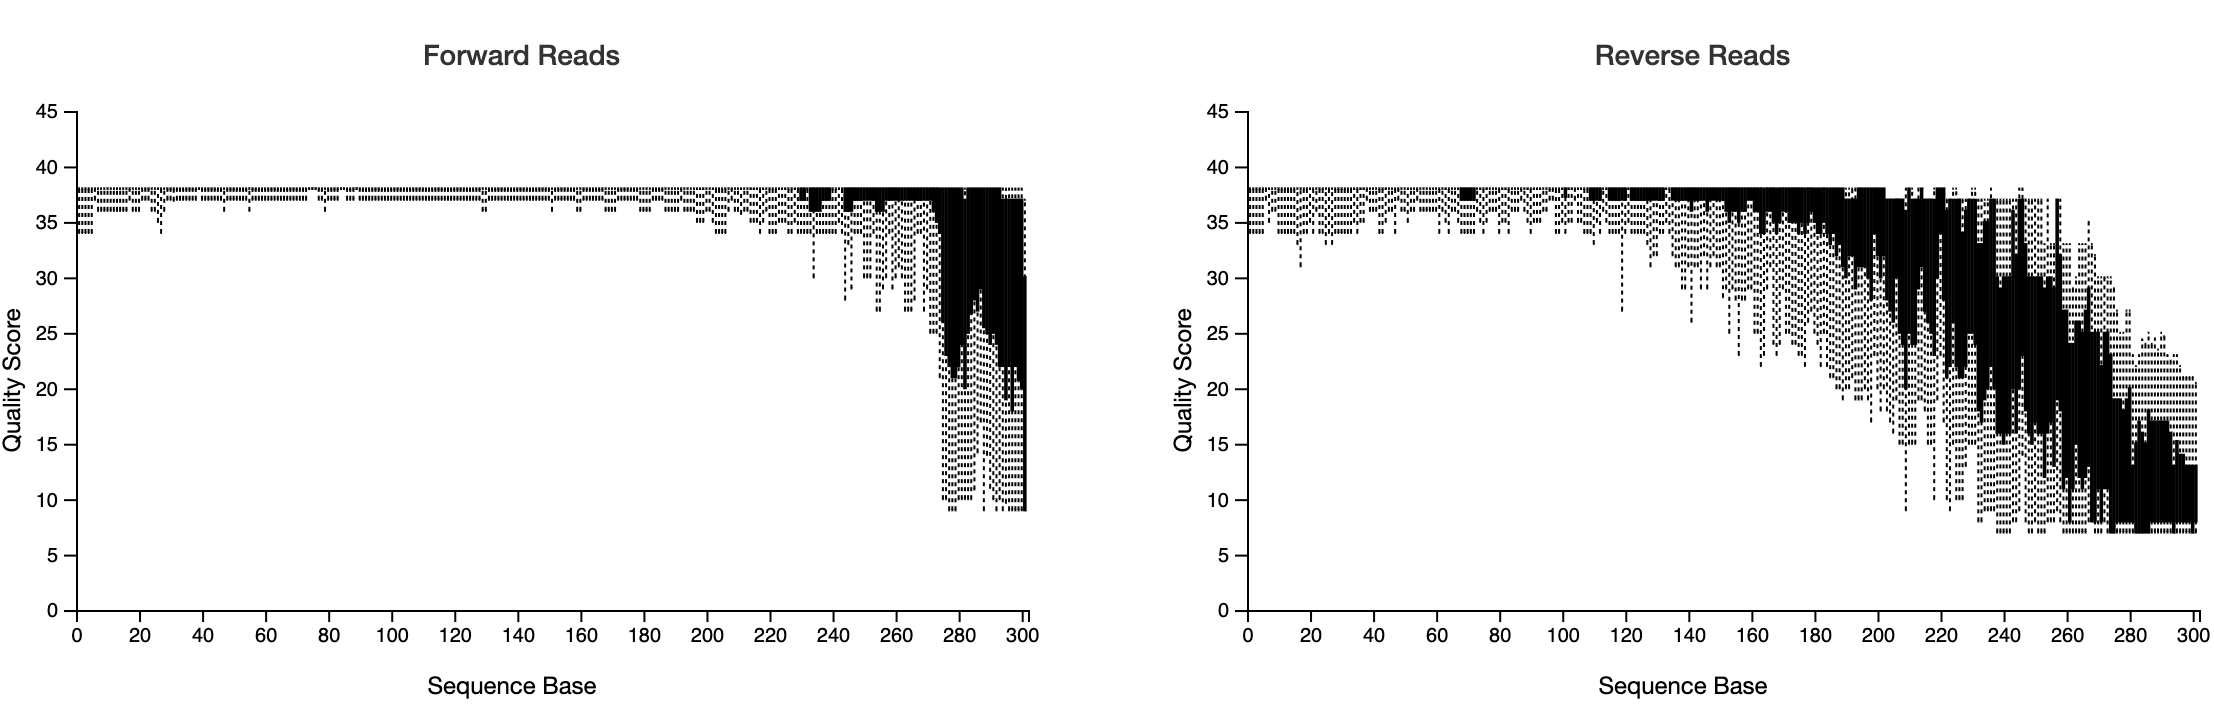
\includegraphics{./img/demux.qza.png}
\caption{``Example of a demux.qzv visualisation''}
\end{figure}

\hfill\break

\textbf{Denoise paired end sequences with dada2 (Step 3)}

Once the trimming and max-ee parameters are decided, it is time to run the DADA2 function. This may take a while, depending on total number of samples.

The output will be a feature\_table.qza and sample\_rep\_seqs.qza, containing the ASV abundances and their sequences respectively.

\begin{verbatim}
qiime dada2 denoise-paired \
  --i-demultiplexed-seqs trimmed_demux-paired-end.qza \
  --o-table feature_table.qza \
  --o-representative-sequences sample_rep_seqs.qza \
  --p-trim-left-f 0 --p-trim-left-r 0 \
  --p-trunc-len-f 271 \
  --p-trunc-len-r 151 \
    --p-max-ee-f 2 \
    --p-max-ee-r 3 \
  --output-dir dada2 \
  --verbose
\end{verbatim}

Summarise and visualise the ASV abundances (feature\_table.qza) in a .qzv file.

\begin{verbatim}
qiime feature-table summarize \
  --i-table feature_table.qza \
  --o-visualization feature_table.qzv \
  --m-sample-metadata-file metadata.tsv
\end{verbatim}

\textbf{Note:} Look at the feature\_table.qzv and record median reads per sample

\begin{figure}
\centering
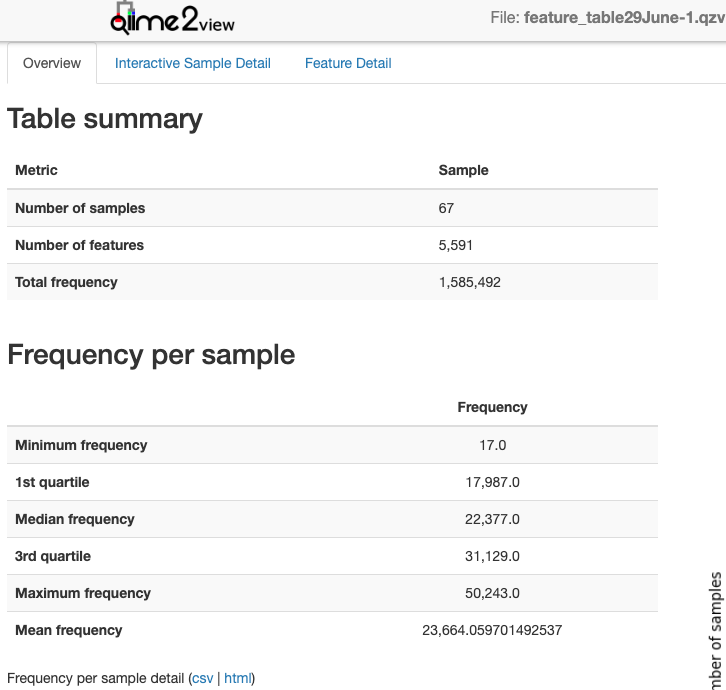
\includegraphics{./img/feature-table.qzv.png}
\caption{``feature\_table.qzv output''}
\end{figure}

\hfill\break

\textbf{Taxonomic classifier and assignment (Step 4)}

The next step is to assign taxonomies to the sequences in the denoised sample sequences. Here, we use a pre-trained classifier that is based on the Silva database. This pre-trained classifier is available on the data resource page of Qiime (Most current link at the time of writing: \url{https://docs.qiime2.org/2022.2/data-resources}).

However, in case you used a different primer you would have to create the classifier yourself. Again there is great resource avaiable on \url{https://docs.qiime2.org}. The process is fairly straight forward but takes computational time. Briefly, extract reference reads from a database (i.e.~Silva here) based on the primers used. Then use those extracted sequences and fit or train them onto a taxonomy. Basically, predict which amplicon sequence should be what phylym/class/order/family/genus etc\ldots. This trained file becomes a `classifier' that is used to assign taxonmies on your sequences.

Here we have a pre-trained classifier, silva-132-99-515-806-nb-classifier.qza:
The output is a file called taxonomy\_silva.qza and taxonomy\_silva.qzv in this case.

\begin{verbatim}
qiime feature-classifier classify-sklearn \
  --i-classifier silva-132-99-515-806-nb-classifier.qza \
  --p-reads-per-batch 10000 \
  --i-reads sample_rep_seqs.qza \
  --o-classification taxonomy_silva.qza \
  --quiet

# Then summarise and visualise the output into a .qza file

qiime metadata tabulate \
--m-input-file taxonomy_silva.qza \
--o-visualization taxonomy_silva.qzv
\end{verbatim}

\textbf{IMPORTANT:} The \texttt{taxonomy\_silva.qzv} is loaded into \url{https://view.qiime2.org/} to dowload the \texttt{.tsv} file for later import into R.

\hfill\break

\textbf{Build phylogenetic tree (Step 5)}

The next step is not essential but really good to have. Creating a phylogenetic tree from the amplicon sequences.

In this case we are using the insertion tree method. See \url{https://library.qiime2.org/plugins/q2-fragment-insertion/16/} for more information in this method.

As not all ASVs will be inserted we will filter the feature\_table.qza again to keep only those ASVs that are in the tree. You will need the reference file from silva or greengenes. In this case we are using \texttt{sepp-refs-silva-128.qza}.

\begin{verbatim}
qiime fragment-insertion sepp \
  --i-representative-sequences sample_rep_seqs.qza \
  --i-reference-database sepp-refs-silva-128.qza \
  --o-tree insertion-tree.qza \
  --o-placements insertion-placements.qza

qiime fragment-insertion filter-features \
  --i-table feature_table.qza \
  --i-tree insertion-tree.qza \
  --o-filtered-table feature_table_insertiontreefiltered.qza \
  --o-removed-table removed_features.qza
\end{verbatim}

Done!

Everything else including further quality filtering happens with \texttt{phyloseq} in R where we will import the following files:
\texttt{feature\_table\_insertiontreefiltered.qza},
\texttt{taxonomy\_silva.qza} and
\texttt{insertion-tree.qza}.

This will be covered in the next chapter.

\textbf{All steps combined}

Copy and paste this into your script file if needed.

\begin{verbatim}
# Manifest Import
qiime tools import --type 'SampleData[PairedEndSequencesWithQuality]' \
  --input-path manifest.tsv \
  --output-path demux-paired-end.qza \
  --input-format PairedEndFastqManifestPhred33V2

# Cutadapt
qiime cutadapt trim-paired \
  --i-demultiplexed-sequences demux-paired-end.qza \
  --p-front-f GTGARTCATCGAATCTTTG \
  --p-front-r TCCTCCGCTTATTGATATGC \
  --o-trimmed-sequences trimmed_demux-paired-end.qza

qiime demux summarize \
  --i-data trimmed_demux-paired-end.qza \
  --o-visualization trimmed_demux-paired-end.qzv

# Denoise
qiime dada2 denoise-paired \
  --i-demultiplexed-seqs trimmed_demux-paired-end.qza \
  --o-table feature_table.qza \
  --o-representative-sequences sample_rep_seqs.qza \
  --p-trim-left-f 0 --p-trim-left-r 0 \
  --p-trunc-len-f 270 \
  --p-trunc-len-r 235 \
  --output-dir dada2 \
  --verbose

# Taxonomic assignment
qiime feature-classifier classify-sklearn \
  --i-classifier silva-132-99-515-806-nb-classifier.qza \
  --p-reads-per-batch 10000 \
  --i-reads sample_rep_seqs.qza \
  --o-classification taxonomy_silva.qza \
  --quiet

# Phylogenetic tree
qiime fragment-insertion sepp \
  --i-representative-sequences sample_rep_seqs.qza \
  --i-reference-database sepp-refs-silva-128.qza \
  --o-tree insertion-tree.qza \
  --o-placements insertion-placements.qza

# Final filtering
qiime fragment-insertion filter-features \
  --i-table feature_table.qza \
  --i-tree insertion-tree.qza \
  --o-filtered-table feature_table_insertiontreefiltered.qza \
  --o-removed-table removed_features.qza
\end{verbatim}

Qiime2 reference:\\
Bolyen E, Rideout JR, Dillon MR, Bokulich NA, Abnet CC, Al-Ghalith GA, Alexander H, Alm EJ, Arumugam M, Asnicar F, Bai Y, Bisanz JE, Bittinger K, Brejnrod A, Brislawn CJ, Brown CT, Callahan BJ, Caraballo-Rodríguez AM, Chase J, Cope EK, Da Silva R, Diener C, Dorrestein PC, Douglas GM, Durall DM, Duvallet C, Edwardson CF, Ernst M, Estaki M, Fouquier J, Gauglitz JM, Gibbons SM, Gibson DL, Gonzalez A, Gorlick K, Guo J, Hillmann B, Holmes S, Holste H, Huttenhower C, Huttley GA, Janssen S, Jarmusch AK, Jiang L, Kaehler BD, Kang KB, Keefe CR, Keim P, Kelley ST, Knights D, Koester I, Kosciolek T, Kreps J, Langille MGI, Lee J, Ley R, Liu YX, Loftfield E, Lozupone C, Maher M, Marotz C, Martin BD, McDonald D, McIver LJ, Melnik AV, Metcalf JL, Morgan SC, Morton JT, Naimey AT, Navas-Molina JA, Nothias LF, Orchanian SB, Pearson T, Peoples SL, Petras D, Preuss ML, Pruesse E, Rasmussen LB, Rivers A, Robeson MS, Rosenthal P, Segata N, Shaffer M, Shiffer A, Sinha R, Song SJ, Spear JR, Swafford AD, Thompson LR, Torres PJ, Trinh P, Tripathi A, Turnbaugh PJ, Ul-Hasan S, van der Hooft JJJ, Vargas F, Vázquez-Baeza Y, Vogtmann E, von Hippel M, Walters W, Wan Y, Wang M, Warren J, Weber KC, Williamson CHD, Willis AD, Xu ZZ, Zaneveld JR, Zhang Y, Zhu Q, Knight R, and Caporaso JG. 2019. Reproducible, interactive, scalable and extensible microbiome data science using QIIME 2. Nature Biotechnology 37: 852--857. \url{https://doi.org/10.1038/s41587-019-0209-9}

  \bibliography{book.bib,packages.bib}

\end{document}
